\documentclass[11pt]{article} %twoside
\usepackage[utf8]{inputenc}
\usepackage[ngerman]{babel}
\usepackage[dvipsnames]{xcolor}
\usepackage{libertine}
\usepackage[a4paper]{geometry}
\usepackage{pdfpages}
\usepackage{parskip}
\usepackage{amsmath, amsthm, amssymb, commath, mathtools}
\usepackage{cancel}
\usepackage{physics}
\usepackage{nicefrac}
\usepackage{booktabs}
\usepackage{tabularx}
\usepackage{tabu}
\usepackage{enumitem}
\usepackage{graphicx}
\graphicspath{{./plots/}{./images/}{./attachments/}}
\usepackage{wrapfig}
\definecolor{capblue}{HTML}{00709B}
\usepackage[margin=1cm,font={small},labelfont={color=capblue}]{caption}
\usepackage{subcaption}
\usepackage{float}
\usepackage{minted}
\usepackage[title]{appendix}
\usepackage{icomma}
\usepackage{multirow}
\usepackage{multicol}
\usepackage[bottom]{footmisc}
\usepackage[separate-uncertainty=true]{siunitx}
\sisetup{locale = DE}
\DeclareSIUnit\pixel{px}
\DeclareSIUnit\pix{px}
% \usepackage{tcolorbox}
\usepackage{titlesec}
\usepackage{ccicons}

\usepackage{csquotes}
\MakeOuterQuote{"}
\renewcommand{\ttdefault}{cmtt}

\usepackage{hyperref}
\usepackage{bookmark}
% https://tex.stackexchange.com/a/33701
\makeatletter
    \newcommand{\nonum}[0]{%
        \let\@oldseccntformat\@seccntformat %
        \renewcommand\@seccntformat[1]{}%
        }
    \newcommand{\resnum}[0]{\let\@seccntformat\@oldseccntformat}
\makeatother

\usepackage{chngcntr}
\counterwithin{figure}{section}

\usepackage[style=iso-authoryear,sortcites=true,sorting=nyt,backend=biber,language=ngerman,natbib=true,sortlocale=de_DE]{biblatex}
\addbibresource{references.bib}
\newcommand{\mkbibbracketscol}[1]{\textcolor{gray}{\mkbibbrackets{#1}}}
\DeclareCiteCommand{\cite}[\mkbibbracketscol]
  {\usebibmacro{prenote}}
  {\usebibmacro{citeindex}%
   \usebibmacro{cite}}
  {\multicitedelim}
  {\usebibmacro{postnote}}

\DeclareCiteCommand{\parencite}[\mkbibbracketscol]
  {\usebibmacro{prenote}}
  {\usebibmacro{citeindex}%
   \usebibmacro{cite}}
  {\multicitedelim}
  {\usebibmacro{postnote}}


\DeclareCiteCommand{\cbx@textcite}[\textcolor{gray}]
  {\usebibmacro{textcite:init}}
  {\usebibmacro{citeindex}%
   \usebibmacro{textcite}}
  {}
  {\usebibmacro{textcite:postnote}}

\DefineBibliographyStrings{ngerman}{%
	bibliography 	= {Literaturverzeichnis},
	andothers		= {u.\,a.\adddot}
}

\let\realcitep\citep
\renewcommand*{\citep}[1]{{\footnotesize\realcitep{#1}}}

\newcommand{\versuch}[0]{Mikroskopie@Home}
\newcommand{\versuchLang}[0]{Mikroskopie mit dem Foldscope}

\hypersetup{
	pdftitle={P3A -- \versuch{} Laborbericht},
	pdfauthor={Yudong Sun},
	bookmarksnumbered=true,
	bookmarksopen=true,
	bookmarksopenlevel=2,
	pdfstartview=Fit,
	pdfpagemode=UseOutlines,
	colorlinks=true,
	linkcolor=MidnightBlue,
	filecolor=magenta,      
	urlcolor=blue,
	citecolor=gray
}
\urlstyle{same}

\usepackage{fancyhdr}
\pagestyle{fancy}
\renewcommand{\sectionmark}[1]{\markright{#1}}
\renewcommand{\subsectionmark}[1]{}
\fancyhf{}
% \fancyhead[RO]{Yudong Sun}
% \fancyhead[LO]{\nouppercase{\rightmark} -- \versuch}
% \fancyhead[LE]{Yudong Sun}
% \fancyhead[RE]{\versuch~ -- \nouppercase{\rightmark} }
\fancyhead[L]{Yudong Sun (mit Schramm)}
\fancyhead[R]{{\small \versuch} \\[-3pt] {\footnotesize \nouppercase{\rightmark}}}
\cfoot{\thepage}

% Custom Defs
\newcommand*{\ra}[1]{\renewcommand{\arraystretch}{#1}}
\newcommand*{\maxi}[1]{\text{max}\left(#1\right)}
\newcommand*{\mini}[1]{\text{min}\left(#1\right)}
\newcommand*{\todo}[1]{\textcolor{red}{TODO: #1}}
\newcommand*{\iu}[1]{\textit{\underline{#1}}}
\newcommand*{\gnuplot}[0]{\texttt{gnuplot}}
\newcommand*{\captionbr}[0]{\\\rule{\textwidth}{0pt}\\\vspace{-\baselineskip}}
\newcommand*{\sigfig}[1]{\hspace{0.5cm}\text{(#1 sig. Zif.)}}
\newcommand*{\pbrace}[1]{\left(#1\right)}
\newcommand*{\sbrace}[1]{\left[#1\right]}
\newcommand*{\bDelta}[1]{\pbrace{\Delta #1}}
\newcommand*{\overbar}[1]{\overline{\raisebox{0pt}[1.2\height]{$#1$}}} % https://tex.stackexchange.com/a/87615
% \newenvironment{beispiel}
%     {\begin{tcolorbox}[title=Beispielrechnung]}
%     {\end{tcolorbox}}
\newcommand*{\tou}[1]{\textcolor{Brown}{#1}}

% \addto\captionsngerman{
%     \let\oldfigname\figurename
%     \renewcommand{\figurename}{[\oldfigname}
%     \let\oldthefig\thefigure
%     \renewcommand{\thefigure}{\oldthefig]}
% } % https://tex.stackexchange.com/a/17490
% https://tex.stackexchange.com/a/101624 new line in caption

% Gaußsche Fehler Erzeuger
\makeatletter
    \newcommand{\gausserror}[2]{% \gausserror{G}{faktoren}
        \sqrt{%
            \@tempswafalse
            \@for\factor:=#2
            \do{
                \if@tempswa+%
                \else%
                    \@tempswatrue%
                \fi%
                \left(\pdv{#1}{\factor}\Delta\factor\right)^2%
            }%
        }
    }
\makeatother
% https://tex.stackexchange.com/a/59912
% https://riptutorial.com/latex/example/28657/loops---repeating-things

% Add quad
\makeatletter
    \newcommand{\addquad}[1]{% \gausserror{G}{faktoren}
        \sqrt{%
            \@tempswafalse
            \@for\factor:=#1
            \do{
                \if@tempswa+%
                \else%
                    \@tempswatrue%
                \fi%
                \left(\Delta\factor\right)^2%
            }%
        }
    }
\makeatother

% rej quad
\makeatletter
    \newcommand{\relquad}[1]{% \gausserror{G}{faktoren}
        \sqrt{%
            \@tempswafalse
            \@for\factor:=#1
            \do{
                \if@tempswa+%
                \else%
                    \@tempswatrue%
                \fi%
                \left(\frac{\Delta\factor}{\factor}\right)^2%
            }%
        }
    }
\makeatother

\newcommand*{\ub}[1]{\underbracket[0.1ex]{#1}}
\newcommand*{\ob}[1]{\overbracket[0.1ex]{#1}}
\newcommand*{\brc}[2]{\mathrlap{\ub{\phantom{#1}}_{#2}}#1}
\newcommand*{\brd}[2]{\mathrlap{\ob{\phantom{#1}}^{#2}}#1}

% for LaTeX https://tex.stackexchange.com/a/25251

\makeatletter
	\newcommand{\smaller}[2]{%
		\begingroup
			\fontsize{\dimexpr\f@size pt-#1pt}{\f@baselineskip}\selectfont
			#2%
		\endgroup
	}
	\newcommand{\bigger}[2]{%
		\begingroup
			\fontsize{\dimexpr\f@size pt+#1pt}{\f@baselineskip}\selectfont
			#2%
		\endgroup
	}
\makeatother

% Title
\title{[\versuch{}] \\ \versuchLang \\ Laborbericht}
\author{Yudong Sun\\Gruppe I4\\%
	{\smaller{2}{In Zusammenarbeit mit Schramm [Gruppe J4]}}}
\date{17. März 2021}

% / Custom Defs

\begin{document}
\includepdf[]{deckblatt.pdf}

% Title
	\maketitle
	\thispagestyle{empty}

	% Einstellungen
	\nonum
	\numberwithin{equation}{section}
	% / Einstellungen

	\begin{center}
		\vfill
		\begin{figure}[h]
			\centering%
			\includegraphics[width=\textwidth]{cover.jpg}
			\captionsetup{labelformat=empty}
			\caption{\textit{Individualisiertes Foldscope}}
		\end{figure}
		\vfill
	\end{center}
% / Title

\newpage
\thispagestyle{plain}

Dieser Laborbericht (Lab Report) enthält alle zwei Teile einer Versuchsabgabe (Laborprotokoll und Auswertung). Da keine Stichwörter zur Vorbereitung in der Versuchsanleitung gibt, gibt es in dieser Abgabe auch keinen Vorbereitungsteil. 

Das Experiment war mit Schramm der Gruppe J4 zusammen durchgeführt. 
\tableofcontents
%  Bibliography
	\renewcommand*{\bibfont}{\raggedright}
	\urlstyle{sf}
	\hypersetup{urlcolor=gray}
	\printbibliography
% / Bibliography

\newpage
\section{Teilversuch 1: Bestimmung des Brechungsindex aus dem Reflexionskoeffizient für polarisiertes Licht}
	Wir berechnen zunächst den Fehler der einzelnen Multimetermessung mit:
	\begin{equation}
		\Delta I = 5\% \text{ Rdg} + 1 \text{ Dgt}
	\end{equation}
	\begin{beispiel}
		Für die erste Messung der Messreihe des senkrechten Fall:
		\begin{align}
			\SI{4.50}{\volt}\times\frac{0.5}{100} + \SI{0.01}{\volt} = \SI{0.0325}{\volt} = \SI{0.04}{\volt} \sigfig{1}
		\end{align}
	\end{beispiel}
	Die Normierung erhält man durch $\tilde{I} = \frac{I}{I_0}$ mit dem Fehler:
	\begin{align}
		\Delta \tilde{I} = \tilde{I}\relquad{I, I_0}
	\end{align}
	wobei $I$ und $I_0$ ensprechend mit $\nicefrac{1}{\text{Verstärkungsfaktor}}$ skaliert ist. Der Fehler der Eingangsintensitäten sind wegen Schwankungen während des Versuchs als $\Delta I_0 = \SI{0.05}{\volt}$ abgeschätzt. 
	\begin{beispiel}
		Für die erste Messung der Messreihe des senkrechten Fall:
		\begin{align}
			\tilde{I} &= \frac{\SI{4.50e-3}{\volt}}{\SI{1.23e-1}{\volt}} = \num{0.0365854} \sigfig{6} \\
			\Delta \tilde{I} &= 
			\frac{\SI{4.50e-3}{\volt}}{\SI{1.23e-1}{\volt}}\sqrt{
				\left(\frac{0.04}{4.50} \right)^2 +
				\left(\frac{0.05}{1.23} \right)^2
			} \notag \\
			&= \num{1.6e-3} \sigfig{2}
		\end{align}
		Somit erhalten wir $\tilde{I} = \num{0.366(16)}$.
	\end{beispiel}
	Um die Reflektionskoeffizienten zu erhalten müssen wir noch den Würzel ziehen ($\zeta = \sqrt{\tilde{I}}$) mit dem Fehler:
	\begin{align}
		\Delta \zeta = \gausserror{\zeta}{\tilde{I}} = \frac{\Delta \tilde{I}}{2\sqrt{\tilde{I}}}
	\end{align} Hier werden immer die genaue Werten von $\Delta \tilde{I}$ und $\tilde{I}$ verwendet, um Rundungsfehler zu vermeiden. 
	\begin{beispiel}
		Für die erste Messung der Messreihe des senkrechten Fall:
		\begin{align}
			\zeta &= \sqrt{\frac{\SI{4.50e-3}{\volt}}{\SI{1.23e-1}{\volt}}} = \num{0.191273} \sigfig{6} \\
			\Delta \zeta &= \frac{1}{2}
			\sqrt{\frac{\SI{4.50e-3}{\volt}}{\SI{1.23e-1}{\volt}}}\sqrt{
				\left(\frac{0.04}{4.50} \right)^2 +
				\left(\frac{0.05}{1.23} \right)^2
			} \notag \\
			&= \num{4e-3} \sigfig{1}
		\end{align}
		Somit erhalten wir $\zeta = \num{0.191(4)}$.
	\end{beispiel}

	Alle weitere Rechnung erfolgen im LibreOffice Calc. Rundung erfolgt mit der Funktion \texttt{ROUNDSIG} bzw. \texttt{ROUND}. 

	\subsection{Senkrechter Fall (Polarisationsfilter bei $\theta = \SI{0}{\degree}$)}
		Mit $\alpha = \frac{\varphi}{2}$:
		\begin{center}
			\begin{tabular}{@{} l  *{8}{l} @{}}
				\toprule
				$\alpha/\si{\degree}$        & \num{5.0} & \num{10.0} & \num{15.0} & \num{20.0} & \num{25.0} & \num{30.0} & \num{35.0} & \num{40.0} \\
				\midrule
				$I/\si{\volt}$               & \num{4.50} & \num{4.70} & \num{4.92} & \num{5.34} & \num{6.05} & \num{6.19} & \num{7.25} & \num{8.34} \\
				$\Delta I/\si{\volt}$        & \num{0.04} & \num{0.04} & \num{0.04} & \num{0.04} & \num{0.05} & \num{0.05} & \num{0.05} & \num{0.06} \\
				Verstärkung $/10^\square$    & \num{3} & \num{3} & \num{3} & \num{3} & \num{3} & \num{3} & \num{3} & \num{3} \\
				$\tilde{I}/\si{\volt}$       & \num{0.0366} & \num{0.0382} & \num{0.0400} & \num{0.0434} & \num{0.0492} & \num{0.0503} & \num{0.0589} & \num{0.0678} \\
				$\Delta\tilde{I}/\si{\volt}$ & \num{0.0016} & \num{0.0016} & \num{0.0017} & \num{0.0018} & \num{0.0021} & \num{0.0021} & \num{0.0025} & \num{0.0028} \\
				\midrule
				$\zeta^{\bot}$               & \num{0.191} & \num{0.195} & \num{0.200} & \num{0.208} & \num{0.222} & \num{0.224} & \num{0.243} & \num{0.260} \\
				$\Delta\zeta^{\bot}$         & \num{0.004} & \num{0.005} & \num{0.005} & \num{0.005} & \num{0.005} & \num{0.005} & \num{0.006} & \num{0.006} \\
				\bottomrule
				\\[-0.5em]
				\toprule
				$\alpha/\si{\degree}$        & \num{45.0} & \num{50.0} & \num{55.0} & \num{60.0} & \num{65.0} & \num{70.0} & \num{75.0} & \num{80.0} \\
				\midrule
				$I/\si{\volt}$               & \num{9.59} & \num{1.152} & \num{1.483} & \num{1.762} & \num{2.184} & \num{2.558} & \num{3.770} & \num{4.36} \\
				$\Delta I/\si{\volt}$        & \num{0.06} & \num{0.007} & \num{0.009} & \num{0.010} & \num{0.012} & \num{0.014} & \num{0.029} & \num{0.04} \\
				Verstärkung $/10^\square$    & \num{3} & \num{2} & \num{2} & \num{2} & \num{2} & \num{2} & \num{2} & \num{2} \\
				$\tilde{I}/\si{\volt}$       & \num{0.078} & \num{0.094} & \num{0.121} & \num{0.143} & \num{0.178} & \num{0.208} & \num{0.307} & \num{0.354} \\
				$\Delta\tilde{I}/\si{\volt}$ & \num{0.004} & \num{0.004} & \num{0.005} & \num{0.006} & \num{0.008} & \num{0.009} & \num{0.013} & \num{0.015} \\
				\midrule
				$\zeta^{\bot}$               & \num{0.279} & \num{0.306} & \num{0.347} & \num{0.378} & \num{0.421} & \num{0.456} & \num{0.554} & \num{0.595} \\
				$\Delta\zeta^{\bot}$         & \num{0.006} & \num{0.007} & \num{0.008} & \num{0.008} & \num{0.009} & \num{0.010} & \num{0.012} & \num{0.013} \\
				\bottomrule
			\end{tabular}
		\end{center}
		Es ist ein Fehler von $\Delta \alpha = \SI{2.5}{\degree}$ zu berücksichtigen.

		Nun tragen wir $\zeta^{\bot}$ gegen $\alpha$ und führe eine Kurveanpassung mit der (modifizierten) Gleichung (8) aus der Anleitung:
		\begin{equation}
			\zeta^{\bot} = \frac{\left(\sqrt{n^2 - \sin^2\alpha} - \cos\alpha\right)^2}{n^2 - 1}
		\end{equation}
		mittles \gnuplot{} durch (Siehe Appendix \ref{appdx:tv1-senk-gp}). Da die Brechungsindex $n$ von Flintglas definitv größer als $1$ ist, muss man hier die in Gleichung (8) stehende $1$ und $n^2$ im Nenner tauschen, sodass man positive Werte erhält. Als Anfangswert ist der Literaturwert\footnote{\href{https://www.rp-photonics.com/flint_glasses.html}{www.rp-photonics.com/flint\_glasses.html}} von $n=\num{1.55}$ verwendet. 
		\begin{figure}[H]
			\centering
			% GNUPLOT: LaTeX picture with Postscript
\begingroup
  \makeatletter
  \providecommand\color[2][]{%
    \GenericError{(gnuplot) \space\space\space\@spaces}{%
      Package color not loaded in conjunction with
      terminal option `colourtext'%
    }{See the gnuplot documentation for explanation.%
    }{Either use 'blacktext' in gnuplot or load the package
      color.sty in LaTeX.}%
    \renewcommand\color[2][]{}%
  }%
  \providecommand\includegraphics[2][]{%
    \GenericError{(gnuplot) \space\space\space\@spaces}{%
      Package graphicx or graphics not loaded%
    }{See the gnuplot documentation for explanation.%
    }{The gnuplot epslatex terminal needs graphicx.sty or graphics.sty.}%
    \renewcommand\includegraphics[2][]{}%
  }%
  \providecommand\rotatebox[2]{#2}%
  \@ifundefined{ifGPcolor}{%
    \newif\ifGPcolor
    \GPcolortrue
  }{}%
  \@ifundefined{ifGPblacktext}{%
    \newif\ifGPblacktext
    \GPblacktexttrue
  }{}%
  % define a \g@addto@macro without @ in the name:
  \let\gplgaddtomacro\g@addto@macro
  % define empty templates for all commands taking text:
  \gdef\gplbacktext{}%
  \gdef\gplfronttext{}%
  \makeatother
  \ifGPblacktext
    % no textcolor at all
    \def\colorrgb#1{}%
    \def\colorgray#1{}%
  \else
    % gray or color?
    \ifGPcolor
      \def\colorrgb#1{\color[rgb]{#1}}%
      \def\colorgray#1{\color[gray]{#1}}%
      \expandafter\def\csname LTw\endcsname{\color{white}}%
      \expandafter\def\csname LTb\endcsname{\color{black}}%
      \expandafter\def\csname LTa\endcsname{\color{black}}%
      \expandafter\def\csname LT0\endcsname{\color[rgb]{1,0,0}}%
      \expandafter\def\csname LT1\endcsname{\color[rgb]{0,1,0}}%
      \expandafter\def\csname LT2\endcsname{\color[rgb]{0,0,1}}%
      \expandafter\def\csname LT3\endcsname{\color[rgb]{1,0,1}}%
      \expandafter\def\csname LT4\endcsname{\color[rgb]{0,1,1}}%
      \expandafter\def\csname LT5\endcsname{\color[rgb]{1,1,0}}%
      \expandafter\def\csname LT6\endcsname{\color[rgb]{0,0,0}}%
      \expandafter\def\csname LT7\endcsname{\color[rgb]{1,0.3,0}}%
      \expandafter\def\csname LT8\endcsname{\color[rgb]{0.5,0.5,0.5}}%
    \else
      % gray
      \def\colorrgb#1{\color{black}}%
      \def\colorgray#1{\color[gray]{#1}}%
      \expandafter\def\csname LTw\endcsname{\color{white}}%
      \expandafter\def\csname LTb\endcsname{\color{black}}%
      \expandafter\def\csname LTa\endcsname{\color{black}}%
      \expandafter\def\csname LT0\endcsname{\color{black}}%
      \expandafter\def\csname LT1\endcsname{\color{black}}%
      \expandafter\def\csname LT2\endcsname{\color{black}}%
      \expandafter\def\csname LT3\endcsname{\color{black}}%
      \expandafter\def\csname LT4\endcsname{\color{black}}%
      \expandafter\def\csname LT5\endcsname{\color{black}}%
      \expandafter\def\csname LT6\endcsname{\color{black}}%
      \expandafter\def\csname LT7\endcsname{\color{black}}%
      \expandafter\def\csname LT8\endcsname{\color{black}}%
    \fi
  \fi
    \setlength{\unitlength}{0.0500bp}%
    \ifx\gptboxheight\undefined%
      \newlength{\gptboxheight}%
      \newlength{\gptboxwidth}%
      \newsavebox{\gptboxtext}%
    \fi%
    \setlength{\fboxrule}{0.5pt}%
    \setlength{\fboxsep}{1pt}%
\begin{picture}(8640.00,5760.00)%
    \gplgaddtomacro\gplbacktext{%
      \csname LTb\endcsname%%
      \put(814,704){\makebox(0,0)[r]{\strut{}$0,1$}}%
      \put(814,1332){\makebox(0,0)[r]{\strut{}$0,2$}}%
      \put(814,1960){\makebox(0,0)[r]{\strut{}$0,3$}}%
      \put(814,2588){\makebox(0,0)[r]{\strut{}$0,4$}}%
      \put(814,3215){\makebox(0,0)[r]{\strut{}$0,5$}}%
      \put(814,3843){\makebox(0,0)[r]{\strut{}$0,6$}}%
      \put(814,4471){\makebox(0,0)[r]{\strut{}$0,7$}}%
      \put(814,5099){\makebox(0,0)[r]{\strut{}$0,8$}}%
      \put(946,484){\makebox(0,0){\strut{}$0$}}%
      \put(1757,484){\makebox(0,0){\strut{}$10$}}%
      \put(2568,484){\makebox(0,0){\strut{}$20$}}%
      \put(3378,484){\makebox(0,0){\strut{}$30$}}%
      \put(4189,484){\makebox(0,0){\strut{}$40$}}%
      \put(5000,484){\makebox(0,0){\strut{}$50$}}%
      \put(5811,484){\makebox(0,0){\strut{}$60$}}%
      \put(6621,484){\makebox(0,0){\strut{}$70$}}%
      \put(7432,484){\makebox(0,0){\strut{}$80$}}%
      \put(8243,484){\makebox(0,0){\strut{}$90$}}%
    }%
    \gplgaddtomacro\gplfronttext{%
      \csname LTb\endcsname%%
      \put(209,2901){\rotatebox{-270}{\makebox(0,0){\strut{}Reflektionskoeffizient $\zeta^\bot$ (Einheitslos)}}}%
      \put(4594,154){\makebox(0,0){\strut{}Einfallswinkel $\alpha$ ($\si{\degree}$)}}%
      \csname LTb\endcsname%%
      \put(7256,1427){\makebox(0,0)[r]{\strut{}$\frac{\left(\sqrt{(1,46469)^2 - \sin^2\alpha} - \cos\alpha\right)^2}{(1,46469)^2 - 1}$}}%
      \csname LTb\endcsname%%
      \put(7256,987){\makebox(0,0)[r]{\strut{}Messpunkte}}%
      \csname LTb\endcsname%%
      \put(4594,5429){\makebox(0,0){\strut{}Reflektionskoeffizient gegen Einfallswinkel}}%
    }%
    \gplbacktext
    \put(0,0){\includegraphics[width={432.00bp},height={288.00bp}]{tv1-senkrecht}}%
    \gplfronttext
  \end{picture}%
\endgroup

			\caption{\centering Reflexionskoeffizient gegen Einfallswinkel $(\chi^2_{\text{red}} = 1.07006 \approx 1 \Rightarrow \text{Gute Anpassung})$ }
			\label{fig:tvone-senk}
			\vspace{-1em}
		\end{figure}
		Als Endergebnis erhalten wir $n = \num{1.46469(659)} = \num{1.465(7)}$. Aus dem Fit ist $\zeta^\bot$ bei senkrechtem Einfall ($\alpha = \SI{0}{\degree}$) gegeben durch:
		\begin{align}
			\zeta^\bot &= \frac{(n-1)^2}{n^2 - 1} = \frac{n - 1}{n + 1} = \frac{\num{1.465} - 1}{\num{1.465} + 1} = \num{0.188641} \sigfig{6} \\
			\Delta\zeta^\bot &= \gausserror{\zeta^{\bot}}{n} = \frac{(n+1)(1) - (n-1)(1)}{(n+1)^2}\Delta n \notag \\
			&= \frac{2\Delta n}{(n+1)^2} = \frac{2(\num{0.007})}{(\num{1.465}+1)^2} = \num{2.4e-3} \sigfig{2}
		\end{align}
		Also erhalten wir $\zeta^\bot(\SI{0}{\degree}) = \num{0.1886(24)}$. Es gibt hier keinen Minimum.

	\subsection{Paralleler Fall (Polarisationsfilter bei $\theta = \SI{90}{\degree}$)}
		Mit $\alpha = \frac{\varphi}{2}$:
		\begin{center}
			\begin{tabular}{@{} l  *{7}{l} @{}}
				\toprule
				$\alpha/\si{\degree}$        & \num{5.0} & \num{10.0} & \num{15.0} & \num{20.0} & \num{25.0} & \num{30.0} & \num{35.0} \\
				\midrule
				$I/\si{\volt}$               & \num{5.49} & \num{5.40} & \num{5.19} & \num{4.77} & \num{4.24} & \num{3.90} & \num{2.983} \\
				$\Delta I/\si{\volt}$        & \num{0.04} & \num{0.04} & \num{0.04} & \num{0.04} & \num{0.04} & \num{0.03} & \num{0.016} \\
				Verstärkung $/10^\square$    & \num{3} & \num{3} & \num{3} & \num{3} & \num{3} & \num{3} & \num{3} \\
				$\tilde{I}/\si{\volt}$       & \num{0.0416} & \num{0.0409} & \num{0.0393} & \num{0.0361} & \num{0.0321} & \num{0.0295} & \num{0.0226} \\
				$\Delta\tilde{I}/\si{\volt}$ & \num{0.0017} & \num{0.0016} & \num{0.0016} & \num{0.0015} & \num{0.0013} & \num{0.0012} & \num{0.0009} \\
				\midrule
				$\zeta^{\parallel}$          & \num{0.204} & \num{0.202} & \num{0.198} & \num{0.190} & \num{0.179} & \num{0.172} & \num{0.1503} \\
				$\Delta\zeta^{\parallel}$    & \num{0.004} & \num{0.004} & \num{0.004} & \num{0.004} & \num{0.004} & \num{0.004} & \num{0.0029} \\
				\bottomrule
				\\[-0.5em]
				\toprule
				$\alpha/\si{\degree}$        & \num{40.0} & \num{45.0} & \num{50.0} & \num{52.5} & \num{55.0} & \num{57.5} & \num{60.0} \\
				\midrule
				$I/\si{\volt}$               & \num{2.477} & \num{1.673} & \num{9.76} & \num{7.20} & \num{3.81} & \num{2.167} & \num{2.466} \\
				$\Delta I/\si{\volt}$        & \num{0.014} & \num{0.010} & \num{0.06} & \num{0.05} & \num{0.03} & \num{0.012} & \num{0.014} \\
				Verstärkung $/10^\square$    & \num{3} & \num{3} & \num{4} & \num{4} & \num{4} & \num{4} & \num{4} \\
				$\tilde{I}/\si{\volt}$       & \num{0.0188} & \num{0.0127} & \num{0.00739} & \num{0.00545} & \num{0.00289} & \num{0.00164} & \num{0.00187} \\
				$\Delta\tilde{I}/\si{\volt}$ & \num{0.0008} & \num{0.0005} & \num{0.00029} & \num{0.00022} & \num{0.00012} & \num{0.00007} & \num{0.00008} \\
				\midrule
				$\zeta^{\parallel}$          & \num{0.1370} & \num{0.1126} & \num{0.0860} & \num{0.0739} & \num{0.0537} & \num{0.0405} & \num{0.0432} \\
				$\Delta\zeta^{\parallel}$    & \num{0.0027} & \num{0.0022} & \num{0.0017} & \num{0.0015} & \num{0.0011} & \num{0.0008} & \num{0.0009} \\
				\bottomrule
				\\[-0.5em]
				\toprule
				$\alpha/\si{\degree}$        & \num{62.5} & \num{65.0} & \num{67.5} & \num{70.0} & \num{75.0} & \num{80.0} & \\
				\midrule
				$I/\si{\volt}$               & \num{4.59} & \num{9.85} & \num{1.907} & \num{4.11} & \num{1.008} & \num{1.677} & \\
				$\Delta I/\si{\volt}$        & \num{0.04} & \num{0.06} & \num{0.011} & \num{0.04} & \num{0.007} & \num{0.010} & \\
				Verstärkung $/10^\square$    & \num{4} & \num{4} & \num{3} & \num{3} & \num{2} & \num{2} & \\
				$\tilde{I}/\si{\volt}$       & \num{0.00348} & \num{0.00746} & \num{0.0144} & \num{0.0311} & \num{0.076} & \num{0.127} & \\
				$\Delta\tilde{I}/\si{\volt}$ & \num{0.00014} & \num{0.00029} & \num{0.0006} & \num{0.0013} & \num{0.003} & \num{0.005} & \\
				\midrule
				$\zeta^{\parallel}$          & \num{0.0590} & \num{0.0864} & \num{0.1202} & \num{0.176} & \num{0.276} & \num{0.356} & \\
				$\Delta\zeta^{\parallel}$    & \num{0.0012} & \num{0.0017} & \num{0.0024} & \num{0.004} & \num{0.006} & \num{0.007} & \\
				\bottomrule
			\end{tabular}
		\end{center}
		Es ist ein Fehler von $\Delta \alpha = \SI{2.5}{\degree}$ zu berücksichtigen.

		Wir bemerken zunächst, dass $\zeta^{\parallel}$ laut der Theorie je nach Einfallswinkel $\alpha$ unterschiedliche Vorzeichen haben. Um das Vorzeichen der experimentellen $\zeta^{\parallel}$-Werten bei dem Fit vernachlässigen zu können, tragen wir nun $\tilde{I} = \left(\zeta^{\parallel}\right)^2$ gegen $\alpha$ anstatt $\zeta^{\parallel}$ und führe eine Kurveanpassung mit der (modifizierten) Gleichung (9) aus der Anleitung:
		\begin{equation}
			\tilde{I} = \left(\zeta^{\parallel}\right)^2 = \left(\frac%
			{n^2\cos(\alpha) - \sqrt{n^2-\sin^2(\alpha)}}%
			{n^2\cos(\alpha) + \sqrt{n^2-\sin^2(\alpha)}}\right)^2
		\end{equation}
		mittles \gnuplot{} durch (Siehe Appendix \ref{appdx:tv1-parl-gp}). Als Anfangswert ist der Literaturwert\footnote{\href{https://www.rp-photonics.com/flint_glasses.html}{www.rp-photonics.com/flint\_glasses.html}} von $n=\num{1.55}$ verwendet. 
		\begin{figure}[H]
			\centering
			% GNUPLOT: LaTeX picture with Postscript
\begingroup
  \makeatletter
  \providecommand\color[2][]{%
    \GenericError{(gnuplot) \space\space\space\@spaces}{%
      Package color not loaded in conjunction with
      terminal option `colourtext'%
    }{See the gnuplot documentation for explanation.%
    }{Either use 'blacktext' in gnuplot or load the package
      color.sty in LaTeX.}%
    \renewcommand\color[2][]{}%
  }%
  \providecommand\includegraphics[2][]{%
    \GenericError{(gnuplot) \space\space\space\@spaces}{%
      Package graphicx or graphics not loaded%
    }{See the gnuplot documentation for explanation.%
    }{The gnuplot epslatex terminal needs graphicx.sty or graphics.sty.}%
    \renewcommand\includegraphics[2][]{}%
  }%
  \providecommand\rotatebox[2]{#2}%
  \@ifundefined{ifGPcolor}{%
    \newif\ifGPcolor
    \GPcolortrue
  }{}%
  \@ifundefined{ifGPblacktext}{%
    \newif\ifGPblacktext
    \GPblacktexttrue
  }{}%
  % define a \g@addto@macro without @ in the name:
  \let\gplgaddtomacro\g@addto@macro
  % define empty templates for all commands taking text:
  \gdef\gplbacktext{}%
  \gdef\gplfronttext{}%
  \makeatother
  \ifGPblacktext
    % no textcolor at all
    \def\colorrgb#1{}%
    \def\colorgray#1{}%
  \else
    % gray or color?
    \ifGPcolor
      \def\colorrgb#1{\color[rgb]{#1}}%
      \def\colorgray#1{\color[gray]{#1}}%
      \expandafter\def\csname LTw\endcsname{\color{white}}%
      \expandafter\def\csname LTb\endcsname{\color{black}}%
      \expandafter\def\csname LTa\endcsname{\color{black}}%
      \expandafter\def\csname LT0\endcsname{\color[rgb]{1,0,0}}%
      \expandafter\def\csname LT1\endcsname{\color[rgb]{0,1,0}}%
      \expandafter\def\csname LT2\endcsname{\color[rgb]{0,0,1}}%
      \expandafter\def\csname LT3\endcsname{\color[rgb]{1,0,1}}%
      \expandafter\def\csname LT4\endcsname{\color[rgb]{0,1,1}}%
      \expandafter\def\csname LT5\endcsname{\color[rgb]{1,1,0}}%
      \expandafter\def\csname LT6\endcsname{\color[rgb]{0,0,0}}%
      \expandafter\def\csname LT7\endcsname{\color[rgb]{1,0.3,0}}%
      \expandafter\def\csname LT8\endcsname{\color[rgb]{0.5,0.5,0.5}}%
    \else
      % gray
      \def\colorrgb#1{\color{black}}%
      \def\colorgray#1{\color[gray]{#1}}%
      \expandafter\def\csname LTw\endcsname{\color{white}}%
      \expandafter\def\csname LTb\endcsname{\color{black}}%
      \expandafter\def\csname LTa\endcsname{\color{black}}%
      \expandafter\def\csname LT0\endcsname{\color{black}}%
      \expandafter\def\csname LT1\endcsname{\color{black}}%
      \expandafter\def\csname LT2\endcsname{\color{black}}%
      \expandafter\def\csname LT3\endcsname{\color{black}}%
      \expandafter\def\csname LT4\endcsname{\color{black}}%
      \expandafter\def\csname LT5\endcsname{\color{black}}%
      \expandafter\def\csname LT6\endcsname{\color{black}}%
      \expandafter\def\csname LT7\endcsname{\color{black}}%
      \expandafter\def\csname LT8\endcsname{\color{black}}%
    \fi
  \fi
    \setlength{\unitlength}{0.0500bp}%
    \ifx\gptboxheight\undefined%
      \newlength{\gptboxheight}%
      \newlength{\gptboxwidth}%
      \newsavebox{\gptboxtext}%
    \fi%
    \setlength{\fboxrule}{0.5pt}%
    \setlength{\fboxsep}{1pt}%
\begin{picture}(8640.00,5760.00)%
    \gplgaddtomacro\gplbacktext{%
      \csname LTb\endcsname%%
      \put(946,704){\makebox(0,0)[r]{\strut{}$0$}}%
      \put(946,1332){\makebox(0,0)[r]{\strut{}$0,05$}}%
      \put(946,1960){\makebox(0,0)[r]{\strut{}$0,1$}}%
      \put(946,2588){\makebox(0,0)[r]{\strut{}$0,15$}}%
      \put(946,3215){\makebox(0,0)[r]{\strut{}$0,2$}}%
      \put(946,3843){\makebox(0,0)[r]{\strut{}$0,25$}}%
      \put(946,4471){\makebox(0,0)[r]{\strut{}$0,3$}}%
      \put(946,5099){\makebox(0,0)[r]{\strut{}$0,35$}}%
      \put(1078,484){\makebox(0,0){\strut{}$0$}}%
      \put(1874,484){\makebox(0,0){\strut{}$10$}}%
      \put(2670,484){\makebox(0,0){\strut{}$20$}}%
      \put(3466,484){\makebox(0,0){\strut{}$30$}}%
      \put(4262,484){\makebox(0,0){\strut{}$40$}}%
      \put(5059,484){\makebox(0,0){\strut{}$50$}}%
      \put(5855,484){\makebox(0,0){\strut{}$60$}}%
      \put(6651,484){\makebox(0,0){\strut{}$70$}}%
      \put(7447,484){\makebox(0,0){\strut{}$80$}}%
      \put(8243,484){\makebox(0,0){\strut{}$90$}}%
    }%
    \gplgaddtomacro\gplfronttext{%
      \csname LTb\endcsname%%
      \put(209,2901){\rotatebox{-270}{\makebox(0,0){\strut{}Reflektionskoeffizient$^2$ $\left(\zeta^\parallel\right)^2$ (Einheitslos)}}}%
      \put(4660,154){\makebox(0,0){\strut{}Einfallswinkel $\alpha$ ($\si{\degree}$)}}%
      \csname LTb\endcsname%%
      \put(7256,4816){\makebox(0,0)[r]{\strut{}$\left(\frac{(1,52605)^2\cos(\alpha) - \sqrt{(1,52605)^2-\sin^2(\alpha)}}{(1,52605)^2\cos(\alpha) + \sqrt{(1,52605)^2-\sin^2(\alpha)}}\right)^2$}}%
      \csname LTb\endcsname%%
      \put(7256,4376){\makebox(0,0)[r]{\strut{}Messpunkte}}%
      \csname LTb\endcsname%%
      \put(4660,5429){\makebox(0,0){\strut{}Reflektionskoeffizient$^2$ gegen Einfallswinkel}}%
    }%
    \gplbacktext
    \put(0,0){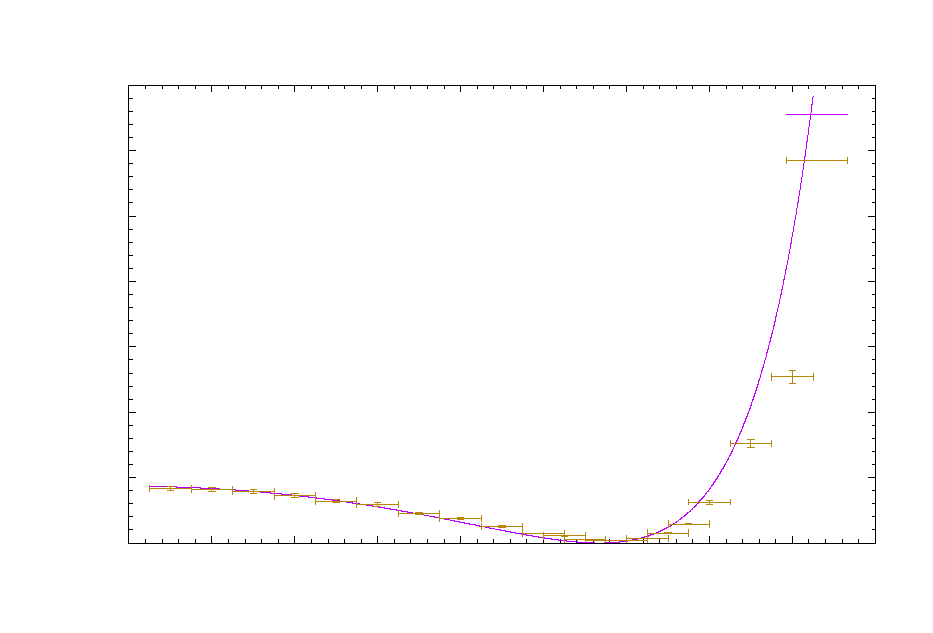
\includegraphics[width={432.00bp},height={288.00bp}]{tv1-parallel}}%
    \gplfronttext
  \end{picture}%
\endgroup

			\caption{\centering Reflexionskoeffizient$^2$ gegen Einfallswinkel $(\chi^2_{\text{red}} = 1.58636 \approx 1 \Rightarrow \text{Gute Anpassung})$ }
			\label{fig:tvone-parl}
			\vspace{-1em}
		\end{figure}
		Als Endergebnis erhalten wir $n = \num{1.52605(879)} = \num{1.526(9)}$. Aus dem Fit ist $\zeta^\parallel$ bei senkrechtem Einfall ($\alpha = \SI{0}{\degree}$) gegeben durch:
		\begin{align}
			\zeta^\parallel &= \frac%
			{n^2 - n}%
			{n^2 + n} 
			= \frac{n-1}{n+1} = \frac{\num{1.526} - 1}{\num{1.526} + 1} = \num{0.208234} \sigfig{6}\\
			\Delta\zeta^\parallel &= \gausserror{\zeta^{\bot}}{n} = \frac{(n+1)(1) - (n-1)(1)}{(n+1)^2}\Delta n \notag \\
			&= \frac{2\Delta n}{(n+1)^2} = \frac{2(\num{0.009})}{(\num{1.526}+1)^2} = \num{2.9e-3} \sigfig{2}
		\end{align}
		Also erhalten wir $\zeta^\parallel(\SI{0}{\degree}) = \num{0.2082(29)}$. Da es schwer ist, um das Minimum aus dem Graphik abzulesen, verwenden wir WolframAlpha\footnote{\href{https://www.wolframalpha.com/input/?i=minimum+of+\%28\%281.526*1.526*cos\%28x\%29-sqrt\%281.526*1.526+-+sin\%28x\%29*sin\%28x\%29\%29\%29+\%2F+\%281.526*1.526*cos\%28x\%29\%2Bsqrt\%281.526*1.526+-+sin\%28x\%29*sin\%28x\%29\%29\%29\%29**2+with+x+from+0+to+1.57}{https://www.wolframalpha.com/input/?i=minimum of ((1.526*1.526*cos(x)-sqrt(1.526*1.526 - sin(x)*sin(x))) / (1.526*1.526*cos(x)+sqrt(1.526*1.526 - sin(x)*sin(x))))**2 with x from 0 to 1.57}}. 

		Wir erhalten somit den Wert $\alpha_p = \SI{0.990699}{\radian} = \SI{56.8}{\degree}$. Es war leider zeitlich schwer, mit dieser Methode auch den Fehler von $\alpha_p$ zu bestimmen. Dazu muss man erst herausfinden, was für ein Effekt die Variation von $n$ auf dem Ergebnis hat. 

		Das gemessene Minimum war bei $\alpha_p = \SI{57.5(25)}{\degree}$. Dieser Wert stimmt mit dem Minimum aus dem Fit überein und der Brechungsindex (und dessen Fehler) daraus ist gegeben durch:
		\begin{align}
			n &= \tan(\alpha_p) = \tan{\SI{57.5}{\degree}/\si{\degree}} = \num{1.56969} \sigfig{6} \\
			\Delta n &= \gausserror{n}{\alpha_p} = (\Delta\alpha_p)\sec^2{\alpha_p} =\frac{\Delta\alpha_p}{\cos^2\alpha_p} \notag \\
			&= \frac{2.5 \cdot \frac{\pi}{180}}{\cos^2(\SI{57.5}{\degree}/\si{\degree})} = \num{0.16} \sigfig{2}
		\end{align}
		Somit erhalten wir $n = \num{1.57(16)}$.
	\subsection{Diskussion}
		Wir berechenen zunächst aus der angegebenen Reflexionskoeffizienten in Tabelle 1 der Anleitung die theoretische Berechungsindex des Flintglases. Es gilt beim senkrechten Einfall ($\alpha = \SI{0}{\degree}$), dass:
		\begin{align}
			\zeta^\parallel = \zeta^\bot = \frac{n-1}{n+1} &= \num{0.240} \notag\\
			n-1 &= \num{0.240}\left(n+1\right) \notag \\
			n(1-\num{0.240}) &= 1+ \num{0.240} \notag \\
			n &= \frac{1+ \num{0.240}}{1 -\num{0.240}} = 1.63 \sigfig{3}
		\end{align}
		Zusammengefasst haben wir aus unseren Ergebnisse vom Teilversuch 1:
		\begin{center}
			\begin{tabular}{ll}
				\toprule
				Methode & $n$ \\
				\midrule
				$\zeta^\bot$      & \num{1.465(7)} \\
				$\zeta^\parallel$ & \num{1.526(9)} \\
				$\alpha_p$        & \num{1.57(16)} \\
				\midrule
				Anleitung         & \num{1.63} \\
				\bottomrule
			\end{tabular}
		\end{center}
		Die experimentelle Werten stimmen miteinander überein, aber nur $n$ aus $\alpha_p$ ist mit der Literaturwert aus der Anleitung verträglich. Hierfür verwenden wir nicht den Literaturwert aus dem Internet, da die Brechungsindizes von Flintgläsern je nach Materie sehr unterschiedlich sind. Wir gehen somit davon aus, dass der Wert aus der Anleitung das richtige Flintglas entspricht. 

		Der Unterschied zwischen den Literaturwert und den experimentell gemessenenen Wert kann vermütlich an den folgenden Fehlerquellen liegen:
		\begin{itemize}
			\item Der Laserstrahl war nicht komplett horizontal, was die Richtung der Polarisation im Vergleich zur Reflektionsebene ändern könnten. Das heißt, dass der senkrechten bzw. parallelen Fall nicht wirklich senkrecht und parallel sind. Das hat zur Folge, dass die Fresnelsche Gleichung nicht komplett anwendbar waren. 
			\item Das Licht im Raum war hell und könnten zur Fehler bei der Messungen führen. Obwohl wir die Nullausgleich gemacht haben, ist der Beitrag von der Raumbeleuchtung je nach Ausrichtung des Prismas unterschiedlich. Da die Beleuchtung auch durch Reflexion polarisiert werden kann, könnte es bei kleiner Messwerten (besonders mit $10^3$ oder $10^4$ Verstärkungen) einen großen Einfluss haben.
			\item Die Polarisationsfilter sind auch nicht perfekt. Wenn die beide Polarisatoren senkrecht stehen, gibt es immer noch ein bisschen Licht, das durch kommt. Dieses Effekt war während des Versuchs leider nicht charakterisiert und deswegen wissen auch nicht, wie dieses Effekt zur unseren Ergebnissen beigetragen haben.
		\end{itemize}

\newcommand*{\nluft}[0]{n_{\text{Luft}}}

\section{Teilversuch 2: Bestimmung des Brechungsindex von Luft}
	Aus der Anleitung ist der Brechungsindex von Luft gegeben durch:
	\begin{equation}
		\nluft = \frac{\lambda P_0}{s}\cdot g + 1 
	\end{equation}
	mit dem entsprechen Fehler:
	\begin{align}
		\Delta \nluft = \nluft \relquad{\lambda,P_0,s,g}
	\end{align}
	wobei $g$ die Steigung des Graphs von $\Delta m$ (die Anzahl der Durchgänge) gegen $P$ (Druck) ist. 

	Wir plotten zunächst die Messwerten und führe mittels \gnuplot{} eine Kurveanpassung der Form $\Delta m = gP + c$ durch (Siehe Appendix \ref{appdx:gnuplottv2}). Ein Messfehler von $\Delta P_i = \SI{1}{\hecto\pascal}$ wird bei der Kurvenanpassung wegen der höhe Anzahl von Messwerten nicht berücksichtigt. 
	\begin{figure}[H]
		\centering
		% GNUPLOT: LaTeX picture with Postscript
\begingroup
  \makeatletter
  \providecommand\color[2][]{%
    \GenericError{(gnuplot) \space\space\space\@spaces}{%
      Package color not loaded in conjunction with
      terminal option `colourtext'%
    }{See the gnuplot documentation for explanation.%
    }{Either use 'blacktext' in gnuplot or load the package
      color.sty in LaTeX.}%
    \renewcommand\color[2][]{}%
  }%
  \providecommand\includegraphics[2][]{%
    \GenericError{(gnuplot) \space\space\space\@spaces}{%
      Package graphicx or graphics not loaded%
    }{See the gnuplot documentation for explanation.%
    }{The gnuplot epslatex terminal needs graphicx.sty or graphics.sty.}%
    \renewcommand\includegraphics[2][]{}%
  }%
  \providecommand\rotatebox[2]{#2}%
  \@ifundefined{ifGPcolor}{%
    \newif\ifGPcolor
    \GPcolortrue
  }{}%
  \@ifundefined{ifGPblacktext}{%
    \newif\ifGPblacktext
    \GPblacktexttrue
  }{}%
  % define a \g@addto@macro without @ in the name:
  \let\gplgaddtomacro\g@addto@macro
  % define empty templates for all commands taking text:
  \gdef\gplbacktext{}%
  \gdef\gplfronttext{}%
  \makeatother
  \ifGPblacktext
    % no textcolor at all
    \def\colorrgb#1{}%
    \def\colorgray#1{}%
  \else
    % gray or color?
    \ifGPcolor
      \def\colorrgb#1{\color[rgb]{#1}}%
      \def\colorgray#1{\color[gray]{#1}}%
      \expandafter\def\csname LTw\endcsname{\color{white}}%
      \expandafter\def\csname LTb\endcsname{\color{black}}%
      \expandafter\def\csname LTa\endcsname{\color{black}}%
      \expandafter\def\csname LT0\endcsname{\color[rgb]{1,0,0}}%
      \expandafter\def\csname LT1\endcsname{\color[rgb]{0,1,0}}%
      \expandafter\def\csname LT2\endcsname{\color[rgb]{0,0,1}}%
      \expandafter\def\csname LT3\endcsname{\color[rgb]{1,0,1}}%
      \expandafter\def\csname LT4\endcsname{\color[rgb]{0,1,1}}%
      \expandafter\def\csname LT5\endcsname{\color[rgb]{1,1,0}}%
      \expandafter\def\csname LT6\endcsname{\color[rgb]{0,0,0}}%
      \expandafter\def\csname LT7\endcsname{\color[rgb]{1,0.3,0}}%
      \expandafter\def\csname LT8\endcsname{\color[rgb]{0.5,0.5,0.5}}%
    \else
      % gray
      \def\colorrgb#1{\color{black}}%
      \def\colorgray#1{\color[gray]{#1}}%
      \expandafter\def\csname LTw\endcsname{\color{white}}%
      \expandafter\def\csname LTb\endcsname{\color{black}}%
      \expandafter\def\csname LTa\endcsname{\color{black}}%
      \expandafter\def\csname LT0\endcsname{\color{black}}%
      \expandafter\def\csname LT1\endcsname{\color{black}}%
      \expandafter\def\csname LT2\endcsname{\color{black}}%
      \expandafter\def\csname LT3\endcsname{\color{black}}%
      \expandafter\def\csname LT4\endcsname{\color{black}}%
      \expandafter\def\csname LT5\endcsname{\color{black}}%
      \expandafter\def\csname LT6\endcsname{\color{black}}%
      \expandafter\def\csname LT7\endcsname{\color{black}}%
      \expandafter\def\csname LT8\endcsname{\color{black}}%
    \fi
  \fi
    \setlength{\unitlength}{0.0500bp}%
    \ifx\gptboxheight\undefined%
      \newlength{\gptboxheight}%
      \newlength{\gptboxwidth}%
      \newsavebox{\gptboxtext}%
    \fi%
    \setlength{\fboxrule}{0.5pt}%
    \setlength{\fboxsep}{1pt}%
\begin{picture}(8640.00,5760.00)%
    \gplgaddtomacro\gplbacktext{%
      \csname LTb\endcsname%%
      \put(814,704){\makebox(0,0)[r]{\strut{}$-90$}}%
      \put(814,1253){\makebox(0,0)[r]{\strut{}$-80$}}%
      \put(814,1803){\makebox(0,0)[r]{\strut{}$-70$}}%
      \put(814,2352){\makebox(0,0)[r]{\strut{}$-60$}}%
      \put(814,2902){\makebox(0,0)[r]{\strut{}$-50$}}%
      \put(814,3451){\makebox(0,0)[r]{\strut{}$-40$}}%
      \put(814,4000){\makebox(0,0)[r]{\strut{}$-30$}}%
      \put(814,4550){\makebox(0,0)[r]{\strut{}$-20$}}%
      \put(814,5099){\makebox(0,0)[r]{\strut{}$-10$}}%
      \put(946,484){\makebox(0,0){\strut{}$10$}}%
      \put(1858,484){\makebox(0,0){\strut{}$20$}}%
      \put(2770,484){\makebox(0,0){\strut{}$30$}}%
      \put(3682,484){\makebox(0,0){\strut{}$40$}}%
      \put(4595,484){\makebox(0,0){\strut{}$50$}}%
      \put(5507,484){\makebox(0,0){\strut{}$60$}}%
      \put(6419,484){\makebox(0,0){\strut{}$70$}}%
      \put(7331,484){\makebox(0,0){\strut{}$80$}}%
      \put(8243,484){\makebox(0,0){\strut{}$90$}}%
    }%
    \gplgaddtomacro\gplfronttext{%
      \csname LTb\endcsname%%
      \put(209,2901){\rotatebox{-270}{\makebox(0,0){\strut{}Drehwinkel $\Psi$ ($\si{\degree}$)}}}%
      \put(4594,154){\makebox(0,0){\strut{}Einfallswinkel $\alpha$ ($\si{\degree}$)}}%
      \csname LTb\endcsname%%
      \put(7256,1427){\makebox(0,0)[r]{\strut{}$\arctan \left(- \frac{\cos\alpha \sqrt{(1,69105)^2-\sin^2\alpha}}{\sin^2\alpha} \right)$}}%
      \csname LTb\endcsname%%
      \put(7256,987){\makebox(0,0)[r]{\strut{}Messpunkte}}%
      \csname LTb\endcsname%%
      \put(4594,5429){\makebox(0,0){\strut{}Drehwinkel der Polarisationsebene gegen Einfallswinkel}}%
    }%
    \gplbacktext
    \put(0,0){\includegraphics[width={432.00bp},height={288.00bp}]{tv2-plot}}%
    \gplfronttext
  \end{picture}%
\endgroup

		\caption{\centering Druck gegen die Anzahl der Durchgängen}
		\label{fig:tv2-plot}
		\vspace{-1em}
	\end{figure}
	Als Ergebnis erhalten wir:
	\begin{center}
		\begin{tabular}{llll}
			\toprule
			Messung & $g/\si{\per\hecto\pascal}$ & $c$ & $\chi^2_\text{red}$ \\
			\midrule
				$1$ & \num{0,12876(67)} & \num{-63,61708(39587)} & \num{0,01169} \\
				$2$ & \num{0,12976(147)} & \num{-65,87209(89462)} & \num{0,05631} \\
				$3$ & \num{0,15166(586)} & \num{-73,36752(333679)} & \num{0,65034} \\
			\bottomrule
		\end{tabular}
	\end{center}
	Gerundet:
	\begin{center}
		\begin{tabular}{lll}
			\toprule
			Messung & $g/\si{\per\hecto\pascal}$ & $c$ \\
			\midrule
				$1$ & \num{0,1288(7)}  & \num{-63,6(4)}\\
				$2$ & \num{0,1298(15)} & \num{-65,9(9)}\\
				$3$ & \num{0,152(6)}   & \num{-73(4)}\\
			\bottomrule
		\end{tabular}
	\end{center}
	Nun berechnen wir den Mittelwert von $g$. Wir vernachlässigen jegliche Fehler bei der einzelnen $g$-Werten und nehmen die statische Schwankung $$\Delta g = \frac{g_{\text{max}} - g_\text{min}}{2}$$ als der Fehler, da diese Schwankung viel große ist. Es ist in diesem Fall wegen der niedrigen Anzahl von $g$-Werten nicht sinnvoll, die Standardabweichung zu nehmen. 

	Wir erhalten somit $\overline{g} = \SI{0.137(12)}{\per\hecto\pascal}$. Im Folgenden ist $g = \overline{g}$.

	Mit der Messwerten:
	\begin{center}
		\begin{tabular}{lll}
			\toprule
			Variable & Wert & Bedeutung \\
			\midrule
			$\lambda$ & \SI{520(20)}{\nano\meter} & Wellenlänge des Lasers \\
			$P_0$ & \SI{9.51(1)e4}{\pascal} & Atmosphäredruck im Raum \\
			$s$ & \SI{256.38(3)}{\milli\meter} & Optische Länge der Küvette \\
			$g$ & \SI{1.37(12)e-3}{\per\pascal} & Durchschnittliche Steigung \\
			\bottomrule
		\end{tabular}
	\end{center}
	erhalten wir:
	\begin{align}
		\nluft 
		&= \frac{(\SI{520e-9}{\meter})(\SI{9.51e4}{\pascal})}{\SI{256.38e-3}{\meter}}\cdot (\SI{1.37e-3}{\per\pascal}) + 1 \notag \\
		&= \num{1.000264253} \sigfig{10} \\
		\Delta\nluft 
		&= (\num{1.000264253}) \sqrt{
			\left(\frac{20}{520}\right)^2 +
			\left(\frac{0.01}{9.51}\right)^2 +
			\left(\frac{0.03}{256.38}\right)^2 +
			\left(\frac{0.12}{1.37}\right)^2
		} \notag \\
		&= \num{0.10} \sigfig{2}
	\end{align}
	Somit erhalten wir als Endergebnis: $\nluft = \num{1.00(10)}$.

	Dieses Ergebnis stimmt mit der Literaturwert $n_\text{Luft, Lit} = 1.000269$ überein. Der Fehler ist aber sehr groß, was hauptsächlich zur
	\begin{itemize}
		\item Unsicherheit in der Wellenlänge des Lasers und
		\item Unsicherheit bei dem selbstständigen Zählen der Durchgängen
	\end{itemize}
	zurückzuführen ist. 
\section{Teilversuch 3: Fraunhofer-Beugung am Einfachspalt}
	Die mögliche Fehlerquellen sind:
	\begin{itemize}
		\item Die Messung der Abstand $R$ war ziemlich ungenau, da es schwer ist, das Mittel des Spaltes per Augenmaß zu bestimmen. Man kann auch schwer feststellen, ob das Maßband senkrecht zum Spalt und CCD-Kamera steht, oder sogar, ob der Spalt überhaupt parallel zur CCD Kamera ist. 
		\item Der Laserstrahl war leicht nach unten gekippt. Deswegen trifft er nicht senkrecht auf der Spalte, was zur Änderung im Beugungsmuster führen kann. 
		\item Die Variablen $b$, $\lambda$ und $R$ haben höhe Korrelationen, da viele Wertepaare das gleiche Verhältnis ergibt. Obwohl wir während des Fits im MATLAB die obere und untere Beschränkungen festgelegt haben, gibt es immer noch viel Spielraum. Beispielsweise ist die gefundene Wellenlänge des Lasers \SI{676.8}{\nano\meter}, was viel länger im Vergleich zu unserem Literaturwert ist. Die Unsicherheiten aus MATLAB sind deswegen ziemlich hoch, mit einer Unsicherheit bei der Fitparameter $b$ von $\approx \pm \SI{48e-4}{\meter}$.
		\item Es könnte auch sein, dass die Umgebungsbeleuchtung nicht gleichmäßig auf der CCD-Kamera fällt, was das Fit-Paramter $c$ nicht berücksichtigen kann.
	\end{itemize}
\section{Videoaufzeichnung}
     Zur Teilversuchen 1 und 2 haben wir eine Videoaufzeichnung vorbereitet. Sie ist unter \textcolor{gray}{\textit{redacted}} ansehbar. 

\resnum
\newpage
\begin{appendices}
	\section{\gnuplot{} Quellcode zur Auswertung von Teilversuch 1}
    \subsection{Senkrechter Fall}
    \label{appdx:tv1-senk-gp}
    {  
        % % Surpress "errors" in minted
        % https://tex.stackexchange.com/a/289068
        \renewcommand{\fcolorbox}[4][]{#4}
        \begin{minted}[linenos,breaklines,autogobble,frame=leftline,framesep=10pt]{gnuplot}
#!/usr/bin/env gnuplot

set term epslatex color size 6in, 4in
set output "tv1-senkrecht.tex"
set decimalsign locale 'de_DE.UTF-8'

set title "Reflektionskoeffizient gegen Einfallswinkel"
set ylabel "Reflektionskoeffizient $\\zeta^\\bot$ (Einheitslos)"
set xlabel "Einfallswinkel $\\alpha$ ($\\si{\\degree}$)"

set mxtics
set mytics
set samples 10000

f(x) = ((sqrt(n**2 - (sin(pi*x/180))**2) - cos(pi*x/180))**2)/(n**2 - 1)

n = 1.55
# (x, y, xdelta, ydelta)
fit f(x) "senkrecht.dat" u 1:2:(2.5):3 xyerrors via n

# Linien
set key bottom right spacing 2

titel = "$\\frac{\\left(\\sqrt{(".gprintf("%.5f", n).")^2 - \\sin^2\\alpha} - \\cos\\alpha\\right)^2}{(".gprintf("%.5f", n).")^2 - 1}$"
plot f(x) title titel lc rgb 'dark-magenta', \
    "senkrecht.dat" u 1:2:(2.5):3 with xyerrorbars title "Messpunkte" pointtype 0 lc rgb 'dark-goldenrod'
        \end{minted}
    }
    mit \texttt{senkrecht.dat}:
    \begin{multicols}{2}
        \begin{minted}[linenos,breaklines,autogobble,frame=leftline,framesep=10pt]{text}
#alpha/deg  Zeta    deltaZeta
5           0,191   0,004
10          0,195   0,005
15          0,200   0,005
20          0,208   0,005
25          0,222   0,005
30          0,224   0,005
35          0,243   0,006
40          0,260   0,006
45          0,279   0,006
50          0,306   0,007
55          0,347   0,008
60          0,378   0,008
65          0,421   0,009
70          0,456   0,010
75          0,554   0,012
80          0,595   0,013
        \end{minted}
    \end{multicols}
    \vspace{-\baselineskip}
    Rohausgabe:
    \begin{minted}[linenos,breaklines,autogobble,frame=leftline,framesep=10pt]{text}
After 3 iterations the fit converged.
final sum of squares of residuals : 16.0509
rel. change during last iteration : -1.47495e-06

degrees of freedom    (FIT_NDF)                        : 15
rms of residuals      (FIT_STDFIT) = sqrt(WSSR/ndf)    : 1.03444
variance of residuals (reduced chisquare) = WSSR/ndf   : 1.07006
p-value of the Chisq distribution (FIT_P)              : 0.378676

Final set of parameters            Asymptotic Standard Error
=======================            ==========================
n               = 1.46469          +/- 0.00659      (0.4499%)
    \end{minted}

    \subsection{Paralleler Fall}
    \label{appdx:tv1-parl-gp}
    {  
        % % Surpress "errors" in minted
        % https://tex.stackexchange.com/a/289068
        \renewcommand{\fcolorbox}[4][]{#4}
        \begin{minted}[linenos,breaklines,autogobble,frame=leftline,framesep=10pt]{gnuplot}
#!/usr/bin/env gnuplot

set term epslatex color size 6in, 4in
set output "tv1-parallel.tex"
set decimalsign locale 'de_DE.UTF-8'

set title "Reflektionskoeffizient$^2$ gegen Einfallswinkel"
set ylabel "Reflektionskoeffizient$^2$ $\\left(\\zeta^\\parallel\\right)^2$ (Einheitslos)"
set xlabel "Einfallswinkel $\\alpha$ ($\\si{\\degree}$)"

set mxtics
set mytics
set samples 10000

f(x) = ((n*n*cos(x*pi/180)-sqrt(n*n - sin(x*pi/180)*sin(x*pi/180))) / (n*n*cos(x*pi/180)+sqrt(n*n - sin(x*pi/180)*sin(x*pi/180))))**2

n = 1.55
# (x, y, xdelta, ydelta)
fit f(x) "parallel.dat" u 1:2:(2.5):3 xyerrors via n

# Linien
set key top right spacing 2

titel = "$\\left(\\frac{(".gprintf("%.5f", n).")^2\\cos(\\alpha) - \\sqrt{(".gprintf("%.5f", n).")^2-\\sin^2(\\alpha)}}{(".gprintf("%.5f", n).")^2\\cos(\\alpha) + \\sqrt{(".gprintf("%.5f", n).")^2-\\sin^2(\\alpha)}}\\right)^2$"
plot f(x) title titel lc rgb 'dark-magenta', \
    "parallel.dat" u 1:2:(2.5):3 with xyerrorbars title "Messpunkte" pointtype 0 lc rgb 'dark-goldenrod'
        \end{minted}
    }
    mit \texttt{parallel.dat}:
    \begin{multicols}{2}
        \begin{minted}[linenos,breaklines,autogobble,frame=leftline,framesep=10pt]{text}
# alpha/deg tilde{I} delta tilde{I}
5           0,0416   0,0017
10          0,0409   0,0016
15          0,0393   0,0016
20          0,0361   0,0015
25          0,0321   0,0013
30          0,0295   0,0012
35          0,0226   0,0009
40          0,0188   0,0008
45          0,0127   0,0005
50          0,00739  0,00029
52,5        0,00545  0,00022
55          0,00289  0,00012
57,5        0,00164  0,00007
60          0,00187  0,00008
62,5        0,00348  0,00014
65          0,00746  0,00029
67,5        0,0144   0,0006
70          0,0311   0,0013
75          0,076    0,003
80          0,127    0,005
        \end{minted}
    \end{multicols}
    \vspace{-\baselineskip}
    Rohausgabe:
    \begin{minted}[linenos,breaklines,autogobble,frame=leftline,framesep=10pt]{text}
After 3 iterations the fit converged.
final sum of squares of residuals : 30.1409
rel. change during last iteration : -8.25091e-16

degrees of freedom    (FIT_NDF)                        : 19
rms of residuals      (FIT_STDFIT) = sqrt(WSSR/ndf)    : 1.25951
variance of residuals (reduced chisquare) = WSSR/ndf   : 1.58636
p-value of the Chisq distribution (FIT_P)              : 0.0500322

Final set of parameters            Asymptotic Standard Error
=======================            ==========================
n               = 1.52605          +/- 0.008781     (0.5754%)
    \end{minted}

\section{\gnuplot{} Quellcode zur Auswertung von Teilversuch 2}
    \label{appdx:tv2-gnuplot}
    {  
        % % Surpress "errors" in minted
        % https://tex.stackexchange.com/a/289068
        \renewcommand{\fcolorbox}[4][]{#4}
        \begin{minted}[linenos,breaklines,autogobble,frame=leftline,framesep=10pt]{gnuplot}
#!/usr/bin/env gnuplot

set term epslatex color size 6in, 4in
set output "tv2-plot.tex"
set decimalsign locale 'de_DE.UTF-8'

set title "Drehwinkel der Polarisationsebene gegen Einfallswinkel"
set ylabel "Drehwinkel $\\Psi$ ($\\si{\\degree}$)"
set xlabel "Einfallswinkel $\\alpha$ ($\\si{\\degree}$)"

set mxtics
set mytics
set samples 10000

f(x) = (180/pi)*atan(-(cos(x*pi/180)*sqrt(n*n - sin(x*pi/180)*sin(x*pi/180)))/(sin(x*pi/180)*sin(x*pi/180)))

n = 1.55
# (x, y, xdelta, ydelta)
fit f(x) "tv2.dat" u 1:2:(2.5):(0.8) xyerrors via n

# Linien
set key bottom right spacing 2

titel = "$\\arctan \\left(- \\frac{\\cos\\alpha \\sqrt{(".gprintf("%.5f", n).")^2-\\sin^2\\alpha}}{\\sin^2\\alpha} \\right)$"
plot f(x) title titel lc rgb 'dark-magenta', \
    "tv2.dat" u 1:2:(2.5):(0.8) with xyerrorbars title "Messpunkte" pointtype 0 lc rgb 'dark-goldenrod'
        \end{minted}
    }
    mit \texttt{tv2.dat}:
    \begin{multicols}{2}
        \begin{minted}[linenos,breaklines,autogobble,frame=leftline,framesep=10pt]{text}
# alpha/deg Psi/deg
15,0        -89,0
20,0        -87,0
25,0        -84,5
30,0        -81,0
35,0        -76,5
40,0        -73,0
45,0        -67,0
50,0        -60,0
52,5        -56,5
55,0        -52,0
57,5        -48,0
60,0        -43,0
65,0        -35,0
70,0        -25,0
75,0        -14,5
80,0        -11,0
        \end{minted}
    \end{multicols}
    \vspace{-\baselineskip}
    Rohausgabe:
    \begin{minted}[linenos,breaklines,autogobble,frame=leftline,framesep=10pt]{text}
After 5 iterations the fit converged.
final sum of squares of residuals : 9.14718
rel. change during last iteration : -1.04167e-06

degrees of freedom    (FIT_NDF)                        : 15
rms of residuals      (FIT_STDFIT) = sqrt(WSSR/ndf)    : 0.780905
variance of residuals (reduced chisquare) = WSSR/ndf   : 0.609812
p-value of the Chisq distribution (FIT_P)              : 0.869697

Final set of parameters            Asymptotic Standard Error
=======================            ==========================
n               = 1.69105          +/- 0.04292      (2.538%)
    \end{minted}
\end{appendices}

\end{document}
